% !TEX TS-program = xelatex
% !TEX encoding = UTF-8 Unicode
% !BIB TS-program = biber

\documentclass[a5paper]{veryshortguide}
\addbibresource{vsg.bib}
\begin{document}
\title{The very short guide to typesetting with~\LaTeX}
\author{Silmaril Consultants\\
  \textbf{Textual Therapy Division}\\
  \protect\url{http://latex.silmaril.ie}}
\date{\monthdate}
\maketitle
\subsection*{What's this all about? What's \LaTeX?}

\LaTeX\ is a document preparation system which uses the \TeX\ typesetting
program. It enables you to produce publication-quality documents with
great accuracy and consistency. \LaTeX\ works on any computer and
produces industry-standard PDF. It is available both
in free (open-source) and commercial implementations. \LaTeX\ can be
used for any kind of document, but it is especially suited to those
with complex structures, repetitive formatting, or notations like
mathematics\footnote{For reasons of space this guide does not cover
  details of mathematics typesetting.}; or where technical stability,
dimensional accuracy, or a persistent and non-proprietary file format
are needed. Install the software from
\url{www.tug.org/texlive/} or buy a commercially-supported
version from one of the vendors (see the list on p.\thinspace\pageref{comm}).

\subsection*{Creating and typesetting your document}

\begin{enumerate}[noitemsep]\setlength{\fboxsep}{1pt}
   \item Create your document using any suitable plain-text editor
     with \LaTeX\ controls, eg \textit{\TeX shop} (Mac), \textit{\TeX
       Maker} (Win), \textit{Kile} (Linux), \textit{Emacs} (all),
     even \textit{vi}\thinspace!
   \item Save the file with a name ending in \verb+.tex+
     (\emph{never} use spaces in filenames!);
   \item Use the {\small\keys{Build}} or {\small\keys{Compile}}
     toolbar button or menu item in your editor to typeset and display
     the document;\label{typeset}
   \item Make any changes needed in your original document and repeat
     step \ref{typeset}.
\end{enumerate}

\subsection*{Syntax (how to type \LaTeX\ commands --- these are the rules)}

\begin{itemize}[noitemsep]
  \item \textbf{All \LaTeX\ commands begin with a backslash}.\\
    \example \verb+\tableofcontents+\endexample
  \item \textbf{If a command needs text to work
    with, it goes in curly braces}.\\
    \example \verb+\title{Irisches Tagebuch}\author{Heinrich Böll}+\endexample
  \item \textbf{If options are used, they go in square brackets
  before the curly braces}.\\
    \example \verb+\documentclass[a4paper,11pt]{book}+\endexample
  \item \textbf{Spaces after commands \emph{without} braces get suppressed}.\\
    \example \verb+Copyright \copyright␣+\texttt{\number\year}
    \gives{Copyright ©\number\year} \nobox\\
    To prevent this, put empty curly braces after the command:\\
    \example \verb+Copyright \copyright{}␣+\texttt{\number\year}
    \gives{Copyright ©~\number\year} \yesbox
  \item \textbf{Curly braces are also used to restrict the scope of
    effects inside them}.\\
    \example \verb+Some {\tiny little} word+ \gives{Some {\tiny little} word}
\end{itemize}
\begin{note}
This guide shows only a tiny fraction of \LaTeX's power. For more
information, visit the \TeX\ Users Group site (\url{www.tug.org}). For
help, see the FAQ (\url{www.tex.ac.uk/faq}), StackExchange
(\url{tex.stackexchange.com}), or the Usenet newsgroup
\url{comp.text.tex}. For packages (plugins), use CTAN, the
Comprehensive \TeX\ Archive Network (\url{www.ctan.org}). For
further details, see \citetitle{fi}
\parencite{fi} and other online resources.
\end{note}

\begin{multicols}{2}\small\parskip4pt
\subsection*{Writing a \LaTeX\ document}
\subsubsection{Basic document structure}

Here's the skeleton of a \LaTeX\ document. These three lines are
\textsc{compulsory}: your document will not work without them:

\begin{Verbatim}[frame=single,fontsize=\small,commandchars=!<>]
!added\documentclass[11pt]{article}
!comment your Preamble goes here (extra setups, if any)
!added\begin{document}
!comment your document text goes here
!added\end{document}
\end{Verbatim}
\vspace*{-.5\baselineskip}
{\fontsize67\selectfont\sffamily New material in each example is shown
in {\ttfamily\added blue}; material from previous examples is in
black. Comments are in \textcolor{DarkRed}{red}.\par}

\begin{itemize}[noitemsep]
  \item The document class name \textsc{must} be one of the standard
    \verb+book+, \verb+article+, or \verb+report+, or one of the many
    others preinstalled or downloadable (eg \verb+thesis+,
    \verb+memoir+, etc);
  \item There are body type size options \verb+10pt+ (the default),
    \verb+11pt+, and \verb+12pt+;
  \item There are paper size options including \verb+a4paper+
    (210\thinspace mm$\times$297\thinspace mm) and \verb+letterpaper+
    (8½$''\times$11$''$) [see below].
\end{itemize}

\subsubsection{Front matter}

The \textbf{Preamble} [see above] is where you speci\-fy any
\textbf{packages} (\LaTeX\ plugins like typefaces or special
formatting), and where you put any changes to standard features.

\begin{Verbatim}[frame=single,fontsize=\small,commandchars=!<>]
\documentclass[a4paper,11pt]{book}
!added\usepackage{charter,graphicx}!revert
!added\setlength{\parindent}{1em}!revert
\begin{document}
!added\title!comment{your document title!revert}
!added\author!comment{your name!revert}
!added\date!comment{date of publication!revert}
!added\maketitle
!added\begin{abstract}
!comment the paragraphs of your abstract go here
!added\end{abstract}
!added\tableofcontents
!comment the text of your document goes here
\end{document}
\end{Verbatim}

The title, author, and date \textsc{must} be followed by the
\verb+\maketitle+ command to be formatted correctly.

\subsubsection{Body matter}

\textbf{Leave a blank line between paragraphs} as you type: this
signals a new paragraph. Spacing is controlled by the
document class and packages you use. For an unindented,
line-spaced style, use the \textsf{parskip} package.

\paragraph{Sectioning:}
Sections get numbered automatically in bold type, and get included in
the Table of Contents (if you use it). Numbering can be turned off
selectively. Section heading layout can be modified with the
\textsf{sectsty}, \mbox{\textsf{titlesec}}, and other packages.

\begin{Verbatim}[frame=single,fontsize=\small,commandchars=!<>]
!comment (Preamble, titling, and abstract as above)
\tableofcontents
!added\chapter!comment{heading of a chapter!revert}
!comment text for the chapter goes here
!added...as shown in section \ref{blah}.
!added\section!comment{heading of a section!revert}
!added\label{blah} !comment make up name for the label
!comment text for the section goes here
!added\chapter!comment{heading of a new chapter!revert}
!comment text for the new chapter goes here
\end{document}
\end{Verbatim}

\paragraph{Lists:}
There are three types of list: \textbf{itemized} (bulleted), \textbf{enumerated} (numbered
or lettered), and \textbf{descriptive} (topic-and-explanation
format).

Like \textsf{document}, these are all \textbf{environments}, using
\verb+\begin{...}+ and \verb+\end{...}+.

\begingroup\fontsize{4.5}{5.5}\selectfont
\renewcommand{\labelitemi}{\textbullet}
\leftmargini=2em
\setlength{\tabcolsep}{3pt}
\begin{tabular}{@{}%
    p{.25\columnwidth}|%
    p{.32\columnwidth}|%
    p{.33\columnwidth}@{}}
\begin{verbatim}
\begin{itemize}
 \item 1lb Sugar
 \item ½pt Cream
 \item Chocolate
 \item 2oz Butter
\end{itemize}
\end{verbatim}
&
\begin{verbatim}
\begin{enumerate}
 \item Mix ingredients
 \item Boil to 112°C
 \item Stir and cool
 \item Pour into dish
\end{enumerate}
\end{verbatim}
&
\begin{verbatim}
\begin{description}
 \item[Fudge] is fun...
 \item[Broccoli] sucks...
 \item[Exercise] is good
  for you if taken daily
\end{description}
\end{verbatim}
\\\hline\scriptsize
\begin{itemize}[noitemsep]
\item 1lb Sugar
\item ½pt Cream
\item Chocolate
\item 2oz Butter
\end{itemize}
&\fontsize{6.5}{8}\selectfont
\begin{enumerate}[noitemsep]
\item Mix ingredients
\item Boil to 112°C
\item Stir and cool
\item Pour into dish
\end{enumerate}
&\tiny
\begin{description}[noitemsep]
\item[Fudge] is fun but fattening if made too often.
\item[Broccoli] sucks, period.
\item[Exercise] is good for you if taken daily and not to extremes.
\end{description}
\end{tabular}
\endgroup

You can nest lists inside each other. Use the \textsf{enumitem}
package to control list formatting.

\colorbox{LightGrey}{\color{black}\begin{minipage}{.965\columnwidth}%
\sffamily\scriptsize\bfseries\raggedright
For help, see the links on the front and back pages. There is a
summary of common commands at\\
\url{www.stdout.org/~winston/latex/latexsheet.pdf}
and a comprehensive list at
\url{www.eeng.dcu.ie/local-docs/latex-help/}~.
\end{minipage}}

\paragraph{Tables and figures:}
These environments \textbf{float} (to fit
available space). They have \verb+\caption+ and \verb+\label+ commands.

\begin{Verbatim}[frame=single,fontsize=\footnotesize,commandchars=!<>]
!added\begin{figure} !comment(see below)
\caption{Swiss and Dutch Mennonite
 migrations of the 1700s and 1800s}
\label{lmig}
!added\centering !comment(centre the contents)
!added\includegraphics[width=.8\columnwidth]
!added {menno-a}\\ !comment(double backslash for linebreak)
!added\scriptsize!revert Courtesy of Paul C. Adams,
 Department of Geography and the
 Environment, University of Texas at
 Austin.
!added\cite{adams}\end{figure}
\end{Verbatim}

Graphics \textsc{must} be EPS files for standard \LaTeX, but JPG, PNG,
or PDF for pdf\LaTeX.

\begin{Verbatim}[frame=single,fontsize=\footnotesize,commandchars=!<>]
!added\begin{table}
 !added\caption{Mean growth rate and intakes
 !added of supplement, milk, and water for 4
 !added diets (after Sherington, J, undated)}
 \label{dietgrowth}
 \centering
 !added\begin{tabular}{|l|r|r|r|r|}
 !added\hline !comment(horizontal line between rows)
  !added&Growth&Supplement&Milk&Water
  !added\\\hline !comment(double backslash for new row)
 !added Supplement&rate&intake&intake&intake
  !added\\\hline
  !added&(g/day)&(g/day)&(ml/kg$^{0.75}$)&
  !added (ml/kg$^{0.75}$)\\\hline
 !added Lucerne &145&450&10.5&144\\\hline
 !added Sesbania&132&476& 9.2&128\\\hline
 !added Leucaena&128&364& 8.9&121\\\hline
 !added None    & 89&  0& 9.8&108\\\hline
 !added\end{tabular}
!added\end{table}
\end{Verbatim}

\begin{center}\sffamily
  \fontsize78\selectfont
\setlength{\tabcolsep}{2pt}
\setlength{\arrayrulewidth}{.2pt}
\begin{tabular}{@{}|>{\vrule height1em width0pt}l|r|r|r|r|@{}}
\multicolumn5l{\textbf{Table 2}: \textit{Mean growth rate and intakes
of supplement,}}\\
\multicolumn5l{\textit{milk, and water for four diets} (after
    Sherington, J, undated)}\\[6pt]\hline
\vrule height1.1em width0pt&Growth&Supplement&Milk&Water\\[-1pt]
Supplement&rate&intake&intake&intake\\[-1pt]
&(g/day)&(g/day)&(ml/kg\textsuperscript{\fontsize34\selectfont 0.75})&(ml/kg\textsuperscript{\fontsize34\selectfont 0.75})\\[3pt]\hline
Lucerne &145&450&10.5&144\\\hline
Sesbania&132&476& 9.2&128\\\hline
Leucaena&128&364& 8.9&121\\\hline
None    & 89&  0& 9.8&108\\\hline
\end{tabular}
\end{center}
Packages like \textsf{longtable} and \textsf{array} can help
with more complex table formats.

\end{multicols}

\begin{center}\sffamily
  \textbf{Figure 1}: \textit{Swiss and Dutch Mennonite migrations of the
    1700s and 1800s}\\[3pt]
  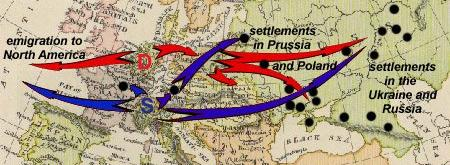
\includegraphics[width=.8\columnwidth]{menno-a}\\\scriptsize
  Courtesy of Paul C. Adams, Department of Geography
  and the Environment, University of Texas at Austin. [1]
\end{center}

\begin{multicols}{2}\small\parskip4pt
\paragraph{Typefaces:}
{\fontfamily{lrm}\selectfont The default typeface in \LaTeX\ is Computer
  Modern, like this.}

{\footnotesize\tabcolsep4pt
\begin{tabular}{@{}l@{\hspace{6pt}}>{\ttfamily}l|l@{\hspace{6pt}}>{\ttfamily}l@{}}
\ff{ptm}Times&mathptmx&\ff{pcr}Courier&courier\\
\ff{ppl}Palatino&mathpazo&\ff{pag}\scriptsize Avant Garde&avant\\
\ff{pbk}Bookman&bookman&\ff{phv}Helvetica&helvet\\
\ff{bch}Charter&charter&\ff{pzc}Zapf Chancery&chancery\\
\ff{put}Utopia&utopia&\ff[OT1]{pnr}Pandora&pandora\\
\ff{pnc}Century&newcent&\ff[U]{yfrak}Fraktur&oldgerm\\
\end{tabular}
}

Dozens of other font packages are available in \TeX\ Live and the \LaTeX\ Font
Catalogue, including mathematics and decorative fonts. Any
Postscript Type~1 font can be configured for \LaTeX.

If you use \XeLaTeX\ and the \textsf{fontspec} package, you can also
use your computer's system fonts as well as those available
with \TeX\ Live.

\colorbox{LightGrey}{\color{black}\begin{minipage}{.965\columnwidth}%
\sffamily\scriptsize\raggedright
Commercial implementations of \TeX\ for Windows with business-level
support are available from Personal \TeX, Inc (PC\TeX); MacKichan
Software, Inc (Scientific Word); Micropress, Inc (V\TeX), and
True\TeX\ Software (True\TeX).\label{comm}
\end{minipage}}

\columnbreak
\textsf{Typefaces continued}

To change font for a word or phrase, use these commands (they can be
nested):

{\small
\begin{tabular}{l@{\enspace}>{\ttfamily\char'134 text}l<{\char'173
      Hello\char'175}@{}>{\ \gives\bgroup}l<{Hello\egroup}}
Italics&it&\itshape\\
Boldface&bf&\bfseries\\
Smallcaps&sc&\ff{cmr}\scshape\\
Sans-serif&sf&\sffamily\\
Monospace&tt&\ttfamily\\
\end{tabular}}

\begingroup\small
\example\verb+\textit{\textbf{\textsf+\linebreak
\verb+{bold italic sans}}}+
\gives{\ff{cmss}\textit{\textbf{bold italic sans}}}
\par\endgroup

Font sizing is automatic for titles, headings, and footnotes. There
are named step-size commands if you need them:

{\scriptsize
\begin{tabular}{>{\ttfamily\char'134}lrrr}
normalsize&10&11&12\\\hline\vrule height1.1em width0pt
tiny&5&6&7\\
scriptsize&6&7&8\\
footnotesize&7&8&9\\
small&9&10&11\\
large&11&12&14\\
Large&12&14&17\rlap*\\
LARGE&14&17\rlap*&20\rlap*\\
huge&17\rlap*&20\rlap*&24\rlap*\\
Huge&20\rlap*&24\rlap*&28\rlap*\\
\end{tabular}
\quad
\rotatebox[origin=c]{90}{\tiny* sizes rounded here to save space}
}

For other sizes, add the special command
{\added\verb+\RequirePackage{fix-cm}+} \emph{before} the
\verb+\documentclass+ line and use
{\added\verb+\fontsize{+\texttt{\uline{pp}}\verb+}{+\texttt{\uline{bb}}\verb+}\selectfont+}
for the point-size (\textit{pp}) and baseline
(\textit{bb}).

{\sffamily\footnotesize
  Size commands are all \textbf{unscoped} commands, so enclose them \emph{and}
the applicable text in curly braces to stop them affecting the rest
of the document.\par}
For double or 1½ line-spacing (eg in theses) use the \textsf{setspace}
package.

You can use colour palettes in the RGB, CMYK, HTML, and other
colourspaces with the
\textsf{xcolor} \\package and the\hfil
\smash{\raisebox{-2ex}{\sffamily\bfseries\Huge\qquad
\textcolor[HTML]{2F50AD}{G}%
\textcolor[HTML]{B32F17}{o}%
\textcolor[HTML]{F3C20B}{o}%
\textcolor[HTML]{2F50AD}{g}%
\textcolor[HTML]{48C847}{l}%
\textcolor[HTML]{B32F17}{e}}}%
\\\verb+\color{+\texttt{\textit{name}}\verb+}+ command.

For verbatim text, use the \verb+\verb+ command or the
\textsf{verbatim} environment, or (better) the \textsf{listings} or
\textsf{fancyvrb} packages, which allow context-sensitive formatting.

\paragraph{Footnotes}\setcounter{footnote}{0}
You can do footnotes with \verb+\footnote(like this}+.\footnote{Like
  this.} Endnotes too.

\paragraph{Cross-references:}\label{blah} Use the command
\verb+\label{...}+ to add a label to the target, and \verb+\ref{...}+ or
\verb+\pageref{...}+ to refer to it. Make up the labels yourself.

\begingroup\small
\example{...\ttfamily section \verb+\ref{blah}+ on
  p.\\ \verb+\pageref{blah}+.}\gives{...section \ref{blah} on
  p.\thinspace\pageref{blah}}.
\par\endgroup

\paragraph{Citation and reference:} Create your bibliographic database
in BIB\TeX\ format \parencite{bibtex} using \emph{JabRef} or
similar. Each entry \textsc{must} have a unique label
(here `\verb+fi+'):\par\vspace{-\parskip}
\begin{Verbatim}[frame=single,fontsize=\scriptsize,commandchars=!<>]
!added@book{fi,
!added  title = {Formatting Information},
!added  author = {Peter Flynn},
!added  publisher = {Silmaril},
!added  year = {2016}}
\end{Verbatim}
\par\vspace{-\parskip}
Use the
\textsf{biblatex} package to specify the style, and give
the filename of your database:\par\vspace{-\parskip}
\begin{Verbatim}[frame=single,fontsize=\footnotesize,commandchars=!<>]
!added\usepackage[style=apa]{biblatex}
!added\addbibresource{myrefs.bib}
\end{Verbatim}
\par\vspace{-\parskip}
To cite, use \verb+\cite{...}+ (or
\verb+\textcite+ or \verb+\parencite+) with the relevant label:\\ \example{\verb+\textcite{fi}+}\gives{\textcite{fi}}.

\subsubsection{Back matter}
For an index, use the \textsf{makeidx} package and the
\verb+\makeindex+ command with the \verb+\index{...}+
and \verb+\printindex+ commands and the \textsf{makeindex} program.

\nocite{*}
{\defbibheading{shortbib}[References]{\subsection*{#1}}\renewcommand*{\bibfont}{\scriptsize}\setlength{\bibhang}{1em}\urlstyle{tt}\label{refs}\printbibliography[heading=shortbib]}

\colorbox{LightGrey}{\color{black}\begin{minipage}{.965\columnwidth}%
\sffamily\scriptsize\bfseries\raggedright
For information about \LaTeX\ training and consutancy, please contact
Silmaril at \url{latex@silmaril.ie}
\end{minipage}}%
\end{multicols}
\end{document}


